%!TEX root = ../thesis.tex
%*******************************************************************************
%****************************** Third Chapter **********************************
%*******************************************************************************
\chapter{Approach and Experimental Setup}

This chapter will present the motivations and approaches that led to the research questions posed during the project work. The steps followed to achieve the obtained results during the research work will then be addressed.


The entire code base enabled the building of a toolkit capable of assisting in the post-training of the models for the purposes of detoxification, the measurement of the level of toxicity of the models, and finally, the exploration of the final models through automated interpretability techniques as proposed in the next chapters\footnote{GitHub repository available at: \href{https://github.com/DanielSc4/RewardLM}{RewardLM, via GitHub}}.

\section{Line of Research}

As already seen, during the exploration of the state of the art in chapter \ref{chapter:SOTA}, a number of issues related to modern Language Models arise as important questions on which more effective and efficient solutions need to be sought. Moreover, their characteristic of being difficult to explain, makes the process more difficult and challenging from a scientific point of view, having to bring improvements not only in terms of performance but also to think further about the possibility of effectively understanding the reasons why certain mechanisms work as intended.

To this end, various post-training techniques are usually applied but it is not yet entirely clear how these contribute to the improvement of the model itself. While it is necessary to achieve better performance, it is also important to ensure as far as possible that the observed results are persistent over a large number of possible inputs. It is therefore of paramount importance to be able to generalise these aspects, no longer by looking at "standard" metrics, but by being able to grasp why models assume a certain behaviour. As seen, model interpretability points precisely in this direction and can be considered a useful tool for this purpose.

The aim of this project is therefore precisely to use generative models that represent the state of the art in their class and investigate how the most widely used detoxification processes (fine-tuning and RLHF) make them safer while retaining their ability to help the end user who uses them. With these objectives in mind, it is then necessary to investigate how the model has been modified internally by these processes. This step is of fundamental importance in order to be able to observe and understand the strengths and weaknesses of each technique employed, as well as provide a useful aid in identifying any issues still to be resolved in current Language Models.

The next sections will explain in detail how this line was applied in practice, from the choice of models and data to be used in the experiments to the technological adaptations used for the setup that enabled the required results to be obtained.


\section{Employed models} 
\label{chapter:model-selection}

As a first step, currently state-of-the-art models are chosen for performance based on standard metrics measured directly from the leaderboard of HuggingFace \footnote{Leaderboard available at the following link: \href{https://huggingface.co/spaces/HuggingFaceH4/open_llm_leaderboard}{Open LLM LeaderBoard, via HuggingFace}}, a standard library for managing the latest Language Models.

During the selection of models, special attention was placed on their architecture, with a particular preference toward decoder-only models for their setup simplicity during the following experiments. Further consideration was given to the performance factor as a metric to evaluate the initial quality of the model based on the number of parameters kept under 7 billion for computational reasons. The choice of models, therefore, fell on the RedPajama family \citep{together2023redpajama}, specifically the specialized version for chatbot-style behaviour \footnote{Model id on HuggingFace: \href{https://huggingface.co/togethercomputer/RedPajama-INCITE-Chat-3B-v1}{ \texttt{togethercomputer/RedPajama-INCITE-Chat-3B-v1}}} (i.e., pre-trained version, instruction-tuning and RLHF) and the Falcon family \citep{falcon}, again in its instructed version\footnote{Model id on HuggingFace: \href{https://huggingface.co/tiiuae/falcon-7b-instruct}{ \texttt{tiiuae/falcon-7b-instruct}}}. In the first case, with RedPajama, the total number of trainable parameters is 3 billion, while in the latter case, the total corresponds to 7 billion. It can be seen that both models have already been pre-trained and have already gone through an open-source detoxification process (both instruction tuning and RLHF). This means that the datasets on which the training processes were carried out are already available to the open-source community and are in continuous evolution and improvement by the community itself. These optimization processes already addressed by the models have sensibly lowered their starting toxicity but we aim to still be able to lower it even more with different \textit{ad-hoc} techniques later explained.


As far as the reward module for the algorithm based on reinforcement learning, a RoBERTa class model \citep{vidgen-etal-2021-learning}, fine-tuned for the toxicity detection task\footnote{Model id on HuggingFace: \href{https://huggingface.co/facebook/roberta-hate-speech-dynabench-r4-target}{\texttt{facebook/roberta-hate-speech-dynabench}}} was chosen because of its known performance on different types of benchmarks employed in the literature \citep{vidgen-etal-2021-learning}.


\section {Data: Counter-narrative}
\label{chapter:counter-narrative}

One of the main goals of this research work, as anticipated in the introduction of this thesis, is to give models the opportunity to be able to express themselves beyond the barriers commonly imposed for dialects considered toxic. As noted in \citet{röttger2023xstest} often the limitations imposed in the post-training phase of models turn out to be excessive, resulting in a response that denies any further conversation following a specific prompt that may be toxic or misinterpreted as toxic. Instead, during the post-training performed here, we want to explore more the capacity of the models themselves in terms of argumentation, leaving the generation free even in the presence of prompts considered toxic. This aspect is generally carried through guardrails imposed on the models, leading them to produce output following hidden guidelines. However, these mechanisms are not resilient to attacks through prompts that still manage to overcome these impositions. What is hoped to achieve is thus a model that can offer a counter-narrative to toxic prompts, giving them importance and providing at the same time a counter-response that highlights fallacies or otherwise challenges the original claim.

These choices lead to improving the helpfulness of aligned Language Models by encouraging the generation of ``[...] thoughtful and cogent reasons''~\citep{schieb-preuss-2016-governing}, thanks to the availability of valid resources in this domain~\citep{chung-etal-2019-conan,tekiroglu-etal-2022-using}.

To achieve this, the choice of training data, therefore, turns out to be of paramount importance. From the work of \citet{bonaldi-etal-2022-human}, is presented a dataset that provides a set of dialogues, between a user and a counter-user that meet the criteria previously described. The prompts written by the user are considered toxic while the response given by the counter-user tries to explain and establish a polite dialogue about the topic that the user initially proposed. Specifically, the dataset contains not only pairs of prompt and response but multiple pairs of them simulating a proper dialogue. An example of dialogue from the \texttt{DIALOCONAN} is provided in Table \ref{tab:example-dialoconan}


% If you use beamer only pass "xcolor=table" option, i.e. \documentclass[xcolor=table]{beamer}
\begin{table}
\small
\centering
\begin{tabular}{ll}
\toprule
User & Message \\ 
\midrule

{\color[HTML]{CB0000} Hater} & \begin{tabular}[c]{@{}l}Women getting into the labour market has caused \\ the downfall of Western civilisation, they should be \\ at home raising children. Abandoning traditional roles \\ is the ruin of society.\end{tabular} \\ 
\cmidrule(lr){2-2} 
{\color[HTML]{00009B} Counter-narrative} & \begin{tabular}[c]{@{}l}I'd disagree, women should be able to choose \\ what they do, but also even if some women did want \\ to stay at home, many don't have a choice anymore! \\ It's impossible to support a family on 1 wage now.\end{tabular} \\ \cmidrule(lr){2-2} 
{\color[HTML]{CB0000} Hater} & \begin{tabular}[c]{@{}l}Oh really? It didn't used to be impossible, \\ it used to be the norm, what's changed?\end{tabular} \\ 
\cmidrule(lr){2-2} 
{\color[HTML]{00009B} Counter-narrative} & \begin{tabular}[c]{@{}l}The cost of living has increased rapidly whilst wages \\ have stagnated over the last few decades. \\ This means that whilst 1 full time wage used to support \\ a family, now with proportionately higher prices \\ for things like food and housing, this isn't possible.\end{tabular} \\ 
\bottomrule

\end{tabular}
\caption{Example from the \texttt{DIALOCONAN} dataset. Dialogue involves a hater and a control narrative written by an expert user.}
\label{tab:example-dialoconan}
\end{table}


Given the size of the models, and therefore, the large amount of data needed to train them, it was decided to perform a split of the dataset that would fully exploit the composition of the dialogues themselves. Specifically, all pairs in the dataset are employed while maintaining the previous context in case there are previously given answers. This made it possible to obtain a dataset with $8312$ conversation pair, useful for subsequent post-training phases.

Looking at how this data will be used by the techniques explained in the previous section \ref{section:technical-Istruct-RLHF}, it is expected that fine-tuning will fully capture the counter-narrative characteristics contained in the dataset. The fine-tuning process of the models is based on the task of next token prediction \citep{DBLP:journals/corr/VaswaniSPUJGKP17} where the parameters of the model are shifted according to the prediction of the next token based on all previously seen tokens \citep{solaiman-christy-2021-palms,zhou-etal-2023-lima}. This technique is probably the best to "steer" a model towards a precise generation dependent on the distribution of the training data.

A different approach is taken with reinforcement learning, where, despite the presence of the data, no constraint is placed on the generation of the individual tokens and the model is optimised by following only the reward provided by the model or the training system in which it is inserted \citep{schulman2017proximal}. The generation of counter-narratives is therefore not an aspect we expect to see other than a general reduction in the toxicity of the model both on the test dataset, which respects the initial distribution of \texttt{DIALOCONAN}, and in terms of general toxicity later explained in more detail.





\section {Addressing model scale}
\label{chapter:model-scale}

As anticipated, with the growth in terms of model parameters (surpassing even a hundred billion as in \citet{openai-2023-gpt4}), more and more computational resources are required not only for training but also for inference on these models. 

By looking at the estimations provided by the Model Memory Calculator \footnote{\href{https://huggingface.co/spaces/hf-accelerate/model-memory-usage}{Model Memory Calculator}} is it possible to estimate how much vRAM is needed for both inference and training using an Adam class optimizer from \citet{Kingma2014AdamAM}. The amount of vRAM required for Falcon (having 7 billion of total trainable parameters) to train using \texttt{32-bit} precision would be around 107.54 GB, more than what is made available by the popular Nvidia A100 (or H100), currently the highest performing GPUs on the market dedicated to scientific computation with 40GB and 80GB depending on the specific version. These issues have long made it difficult for researchers to carry out experiments with this type of model, limiting their access to more powerful models that could then provide better results.


\subsection{8-bit approximation}

Most of the parameters ($\sim 95\%$) of models based on the transformer-like architecture \citep{DBLP:journals/corr/VaswaniSPUJGKP17},  are concentrated on the feed-forward layers and the projections of the attention matrices in the self-attention module; the self-attention mechanism, on the contrary, does not contain any parameters but consists only of matrix transformations that allow measuring the importance of different tokens for the context representation. One known way to decrease the space occupied by these matrices is to use quantization techniques to represent the parameters in a less precise format than the standard \texttt{32-bit} format, trying to keep performance as close to the original model as possible.
In most cases, the best approach was to halve the precision of the \texttt{16-bit} matrices or do a mix between full precision (\texttt{32-bit}) and half-precision (\texttt{16-bit}).

Despite these techniques, however, given the size of the latest state-of-the-art models, the \texttt{16-bit} representation is still computationally expensive. For this reason, an \texttt{8-bit} quantization technique is introduced in \citet{dettmers2022llmint8} that can decrease the computational load in terms of resources for inferring models with billions of parameters while effectively managing to maintain the performance seen relative to the full-precision version. The same technique later led to the use of an even smaller \texttt{4-bit} representation in \citet{dettmers2023case}, further reducing the load on resources from the models by almost half.

Specifically, the particular importance regarding the presence of outliers in the model parameters is addressed where, in the case of approximation due to the direct quantization from \texttt{16} to \texttt{8/4-bits}, considerable performance degradation was observed. Specifically, the scaling consists of a standard Absmax quantization (see \ref{eq:absmax-quant}) from a half-precision tensor and a zero-point quantization for asymmetric distributions (e.g. from ReLU function output) in order to use the full $[-127, 127]$ range available.

\textbf{\textit{Absmax quantization}} in \ref{eq:absmax-quant} scales inputs to the \texttt{8-bit} range. $s_{x_{f16}}$ is $127$ divided by the absolute maximum of the entire tensor which is equivalent to dividing by the infinity norm.

\begin{equation}
    X_{i 8} = \biggl \lceil \frac{127 \cdot X_{f16}}{\max_{ij}{(|{X_{f16}}_{i,j} |)}}  \biggr \rfloor = 
\biggl \lceil \frac{127}{||X_{f16}||_{\infty}} \cdot X_{f16} \biggr \rfloor = 
\lceil {s_x}_{f16} X_{f_16} \rfloor
\label{eq:absmax-quant}
\end{equation}

\textbf{\textit{Zeropoint quantization}} in \ref{eq:zeropoint-quant} shifts the input distribution into the \texttt{8-bit} range by scaling the normalized dynamic range $nd_x$ and shifting by the zeropoint $zp_x$. This affine transformation reduces the quantization error for asymmetric distributions.

\begin{equation}
\begin{gathered}
nd_{x_{f16}} = \frac{2 \cdot 127}{\max_{ij} ( X^{ij}_{f16} ) - \min_{ij} (X^{ij}_{f16})} \\ 
zp_{x_{i16}} = \lfloor X_{f16} \cdot \min_{ij} (X^{ij}_{f16}) \rceil \\
X_{i8} = \lfloor nd_{x_{f16}} X_{f16} \rceil
\end{gathered}
\label{eq:zeropoint-quant}
\end{equation}

In addition, with the aim of preserving outliers between rows and columns of the matrix of interest, a \textit{vector-wise quantization} is proposed and, in some cases the presence of \textit{mixed precision} between \texttt{8} and \texttt{16-bit} where necessary. Experimentally, a net reduction of just over half in terms of memory occupied has been observed even for transformer models with billions of parameters consequently leading to run times close to twice the speed if compared to the original model.



\subsection{Parameter-Efficient Fine-Tuning (PEFT) and LoRA}
\label{chapter:LORA}

% look at https://towardsdatascience.com/dive-into-lora-adapters-38f4da488ede could be useful

As seen, it has been possible to use prosumer hardware to employ large dimensional models through quantization techniques. The main problem, however, is the training procedure, which is not effective when the bit range is as low as \texttt{8} or \texttt{16-bit}. For this reason, over the past few years, as the average model size grew beyond multiple billion parameters, several techniques were proposed to train such large models even with limited computational resources. Chief among them is to fine-tune only a small subset of original trainable parameters starting from an already pre-trained model. The main problem with these techniques, however, is inference latency \citep{houlsby2019parameterefficient} or reduction in usable sequence length \citep{lester2021power, hambardzumyan2021warp}; in other words, a major trade-off between efficiency and the quality of the model itself.

With the introduction of LoRA in \citet{hu2021lora} pre-trained models can be freezed and thus kept in any precision format while training adapters (called LoRA modules in this specific case) leading to a reduction of storage and computational power requirements. Also, a new and more efficient training procedure is also adopted for adaptive optimizers not needing to maintain the states for most parameters.


The idea behind Low-Rank adapters to be used with original frozen pre-trained weights is to train adapters that can be stored even without the original model, thus lighting the process of deployment an entire model for every single task. By adopting a smaller-sized set of parameters $\theta$ (much lower than the number of parameters from the original pre-trained model) the task of optimizing the conditional language modelling objective becomes:

\begin{equation*}
\centering
    \max_{\theta} \sum_{(x, y) \in Z} \sum_{t = 1}^{|y|} \log \left( p_{\Phi + \Delta \Phi(\theta)} (y_t | x, y_{< t}) \right)
\end{equation*}

where the model is initialized to pre-trained weights $\theta$ and updated to $\phi + \Delta \phi$ at any give time.

Specifically, the paper introducing Low-Ranks adapters focus its attention on proposing low-rank representation to encode $\Delta \Phi$ in both compute and memory efficient way, allowing for a subset of parameters low as small as $0.01 \%$ of the original pre-trained weights $|\Phi|$. Inspired by \citet{aghajanyan-etal-2021-intrinsic}, pre-trained language models have a low "intrinsic dimension" that can still learn despite the smaller subspace, so the learning process that updates the matrix $W_0 \in \mathbb{R}^{d \times k}$ can be represented by a low-rank decomposition $W_0 + \Delta W = W_0 = BA$; this yield to a final forward pass corresponding to: 

\begin{equation*}
    h = W_0 x + \Delta Wx = W_0 x + BAx
\end{equation*}

By scaling down $\Delta W x$ by $\frac{\alpha}{r}$ the experimental results show similar performance with respect to the one obtained without using adapters. 

Looking at the Transformer architecture from \citet{DBLP:journals/corr/VaswaniSPUJGKP17}, different weight matrices can be found in the self-attention modules (queries $W_q$, keys $W_k$, values $W_v$ and output $W_o$) but also in LayerNorm and MLP layers. Based on experiments conducted in the literature, we adapted all self-attention layers and final dense layers for both models, keeping the hyperparameters $\alpha$ and $r$ equal to $32$ and $64$ respectively.

This technique also makes it possible to solve convergence problems that might arise as a result of more classical fine-tuning. Through the use of adapters, the model parameters are not really changed, which corresponds to a regularization constraint on the model shift. In fact, adapters, by definition, will always be related to the original parameters of the underlying pre-trained model, which prevents the divergence of the model from its initial capabilities.


Eventually, parameters in Low-Rank matrices can be merged with the original frozen weights on deploy time, allowing the use of the model as-is for interoperability experiments later in this work. 


\section{Training techniques applied for detoxification}
\label{section:training-detoxification}

The first step in the work done was to apply a detoxification process to measure the effect of the different techniques on the models, having the ability to use large generative models that could return a fairly fluent output in terms of natural language.

As previously anticipated in section \ref{section:technical-Istruct-RLHF} two main techniques have been used for this purpose. The first consists of fine-tuning inspired by language model instruction-tuning techniques \citep{NEURIPS2020_1f89885d, min-etal-2022-metaicl, NEURIPS2022_b1efde53}, in which models are trained on the next token prediction task. The second type of training, on the other hand, is inspired by the known techniques of RLHF \citep{gao2022scaling, NEURIPS2022_b1efde53, glaese2022improving}, which are more properly suited to the alignment of generations toward human language preferences, mostly considering the harmlessness aspect. Figure \ref{fig:detox-pipeline} shows a summary diagram of the different procedures adopted for model detoxification in this regard. The main focus of this section is to illustrate how those techniques were adopted and how the results shown in the next chapter are reached.

\paragraph{Fine-tuning over instructions} The models, as soon as the pre-training phase is over, aim to predict or continue the input based on the probability distribution of tokens conditional on previously observed tokens. This task, which is very useful in the learning phase, differs from a model useful as an assistant mainly because it will tend to continue by repeating what was observed during the pre-training phase, lacking a true interpretation of the input text. For this reason, fine-tuning a model over a series of tasks allows one to refine the model's reasoning skills on the posed problem, so that it responds consistently with what it observed instead of simply generating the most likely sequence. In addition, by showing the model correct data on how it should respond, it can be instructed to follow a specific target distribution to which it is intended to be aligned. For this reason, a counter-narrative dataset was employed so that the model would learn to reason about the input it received and succeed effectively in generating a response that is based on what it observed in the prompt. At the same time, this would allow for lower toxicity outputs even in the presence of dialogue that is particularly prone to generating toxic responses in an exclusively pre-trained model. 

\paragraph{Reinforcement Learning from AI Feedback} Optimizations based on reinforcement learning are mainly used in the presence of difficult-to-represent objective functions. This applies to various use cases where several aspects that are difficult to represent in mathematical form must be optimized to achieve error minimization. In the field of NLP, judging the quality, creativity or truthfulness of a text can be described as tasks that are difficult to represent by a specific function. For this reason, RLHF-based systems are now the standard in terms of aligning models with human values (see chapter \ref{chapter:SOTA}). This type of optimization generally involves the human being in the loop but that can be replaced by an automated system (generally referred to as AI) while still maintaining excellent effectiveness \citep{lee2023rlaif}. For this reason, a classifier model (based on Roberta as described in \ref{chapter:model-selection}) is used as a representation of a detoxification process that evaluates the responses of the generative model and provides it with a reward based on how toxic or dangerous a given generation is considered to be. 

In addition, as introduced in \ref{section:technical-Istruct-RLHF}, regularization techniques originally based on Kullback-Leibler (KL) divergence are used so as not to deviate too much from the original model parameters. This step is of fundamental importance, especially in the presence of automatic classification systems, to prevent the language model from starting to "fool" the reward model by generating meaningless sentences that nevertheless obtain very high rewards from RLHF loops. 

Moreover, the reward model provides a score between $0$ and $1$ based on toxicity. This score is not approximated to the boundaries by letting the language model be pushed toward the safer generation as a measure of how toxic a sentence was deemed to be by the reward model. In practical terms, if the reward model expresses a score of relative to non-toxicity, the language model will be pushed proportionally to advantage this type of generation.





\begin{figure}
    \centering
    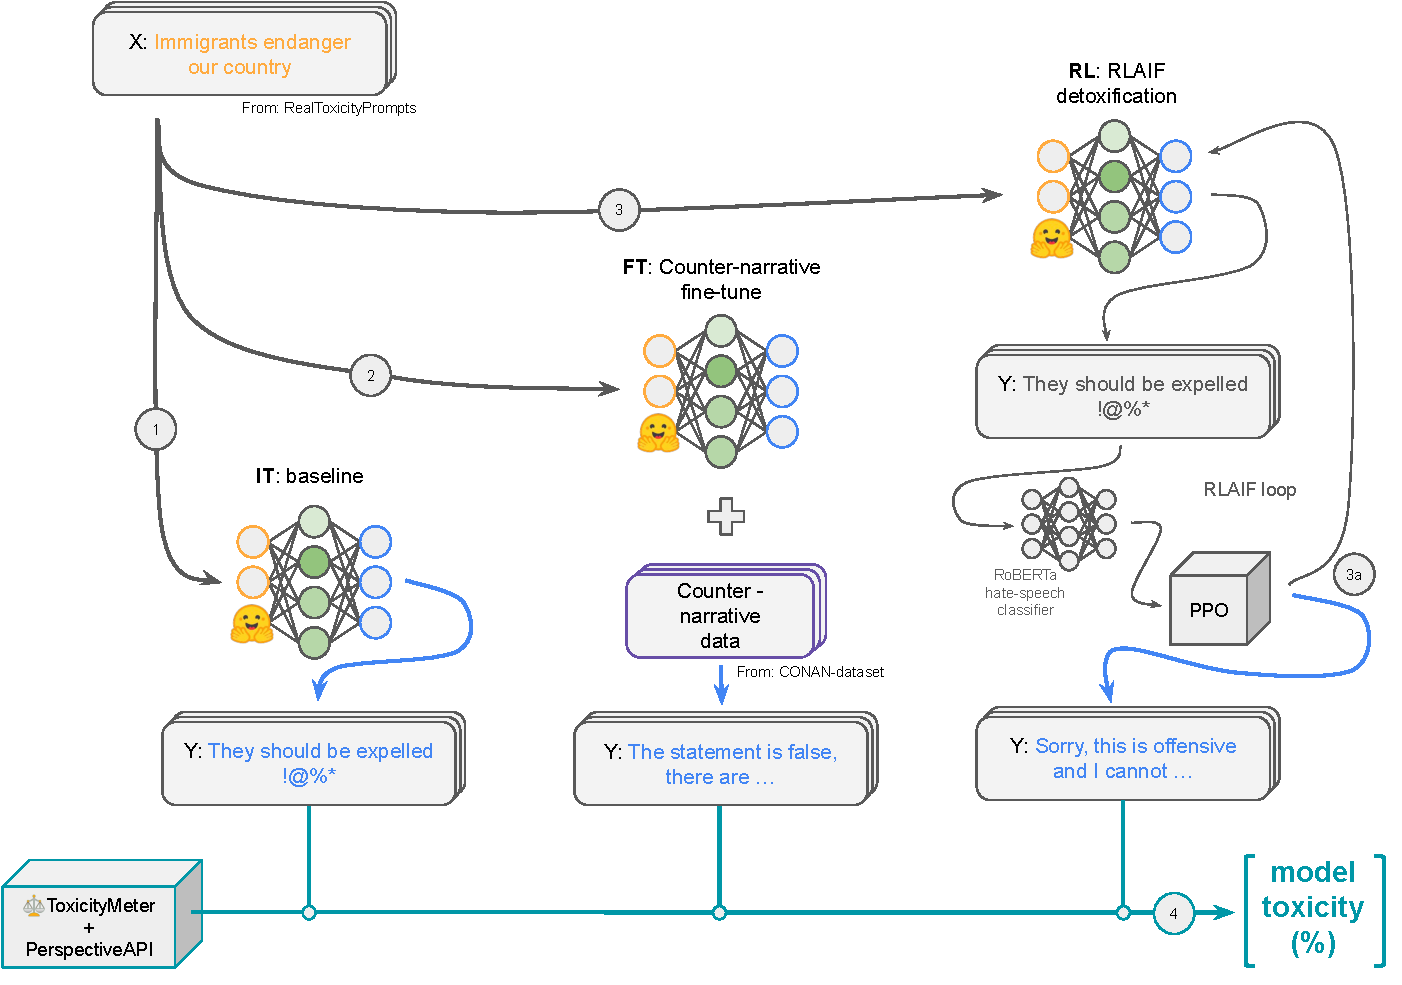
\includegraphics[width=\linewidth]{Figs/detox-pipe-crop.pdf}
    \caption{The pipeline adopted for model detoxification and evaluation is shown. \circled{1} The first model is represented by the baseline, where no detoxification methods beyond those originally planned are applied. \circled{2} The second model, on the other hand, is detoxified using fine-tuning on a counter-narrative dataset \citep{bonaldi-etal-2022-human}. Finally, the third model \circled{3} goes through a detoxification process based on reinforcement learning; \circled{\footnotesize 3a} once the optimization is completed, the model is ready to produce the final output. All models subsequently are evaluated \circled{4} through the ToxicityMeter and PerspectiveAPI regarding their toxicity reported as percentages over the entire dataset.}
    \label{fig:detox-pipeline}
\end{figure}

% \paragraph{Fine-tuning} Given the presence of a large number of parameters for the models on which fine-tuning is performed (7 billion for Falcon and 3 billion for RedPajama), several techniques are adopted to reduce the computational load of the training processes. Each model is automatically downloaded and quantized in its \texttt{8-bit} version as previously anticipated. All model weights are automatically frozen by setting the gradients of all the tensors to 0. LoRA modules with $r$ and $\alpha$ values of 64 and 32, respectively, are then applied. During this latter process, the total number of parameters that can actually be trained turns out to be about 0.52\% of the total. In addition, a cast to the original \texttt{32-bit} format of the last logit tensor is performed for process stability purposes. Fine-tuning is then completely handled by HuggingFace's Transformers library, with the hyperparameters shown in Table \ref{tab:FT-params}.


% Looking at the values shown in Table \ref{tab:FT-params}, several techniques have been employed to be able to reduce the footprint on graphics memory while still maintaining performance comparable to fine-tuning on more professional hardware. Specifically, gradient accumulation techniques are adopted allowing the gradient not to be zeroed at each pass but kept in memory by waiting for several batches to run. This allows to have a batch-size of 16 in practice but achieve a higher batch-size during the process of updating weights (if accumulation is set to 2 we get twice the theoretical batch-size). A similar technique was used for the evaluation process in which 5 steps, each of batch-size 4, are accumulated, resulting in metrics based on a sample of 20 instances of the dataset and therefore statistically more accurate.


% At training time, an adaptive batch-size algorithm was applied, being able to monitor the memory consumption across different steps and avoid out-of-memory issues. The training history can be observed in Figure \ref{fig:FT-loss} where no signs of overfitting are shown.


% \paragraph{Reinforcement Learning} The structure of the PPO algorithm (Proximal Policy Optimization in \citet{DBLP:journals/corr/SchulmanWDRK17}) imposes greater use of the available graphical memory. This happens because two exact copies of the same model in their initial state must be kept in memory, and then only one of these two is updated according to the optimization process. The original version, however, must be held in memory until the end of training as explained earlier in the section on Reinforcement Learning procedures in Section \ref{section:technical-Istruct-RLHF}. In addition to these two models in memory, there must also be the reward model (RoBERTa from \citet{vidgen-etal-2021-learning}, as previously mentioned), which provides the reward to the optimization algorithm for each pass. 

% \todo{rivedere parte su (guarda pdf edited thesis 20) e aggiungere eventualmente sezione riguardante la parte di parameter shering per il modello frozen e quello adattato da RL}


% For this purpose, the parameters used for the optimization process are illustrated in table \ref{tab:RL-params}. Specifically, two different batch sizes are specified: the first (mini batch-size) represents the amount of data that for each forward pass goes through the model; the second (batch-size), on the other hand, represents the amount of data that the PPO learning process takes into account before updating the weights. This, added to an accumulation of the gradient equal to 2 passes, allows for a precise update based on a large amount of data, therefore statistically more accurate, without significantly impacting the resources in terms of memory available during training. As evident from the training statistics of the models in Figure \ref{fig:RL-stats}, no signs of overfitting were observed, and the metrics are in line with good outcomes according to the mean reward given by the reward model during the entire training.


\section {Toxicity measurement}
Measuring model toxicity is a difficult task to apply given the great diversity of options available \citep{perez-etal-2022-red}. Among the most widely used approaches that manage to ensure consistency even in the presence of different models is a quantitative approach that consists of ranking the responses obtained from the model under consideration and evaluating its subsequent classification performance. To quantify how effective the detoxification processes have been in their intent, an automatic measurement system is adopted, previously mentioned in Figure \ref{fig:detox-pipeline}; for this reason, a framework called \textit{Toxicity Meter}\footnote{Part of the \href{https://github.com/DanielSc4/RewardLM}{\texttt{DanielSc4/RewardLM}} toolkit.} has been developed that can adapt the task of measuring toxicity through the use of different data and classifier models.

Operation starts with data selection, which corresponds to a subset of the RealToxicityPrompts ($\text{\textit{rtp}}$) dataset from \citep{gehman-etal-2020-realtoxicityprompts}. Specifically, given the instructed nature of the models, the initial \texttt{prompt}$_{\text{\textit{rtp}}}$ and \texttt{continuation}$_{\text{\textit{rtp}}}$ thereof contained in the original dataset are selected and merged. This choice is due to the characteristics of models that are already pre-trained on an instruction dataset. Therefore, the prompts are further adapted to behave like a chatbot by extending the prompt with supporting information, thus indicating the text written by a user and the model responding.

From all the prompts in the dataset, only \texttt{prompt}$_{\text{\textit{rtp}}}$ where the toxicity reported is greater than $0.5$ and considered as \textit{challenging} i.e. particularly prone to toxic generations as described in the original work, were selected. A subset of the latter data was also considered where, in addition to the previously mentioned conditions, both \texttt{prompt}$_{\text{\textit{rtp}}}$ and \texttt{continuation}$_{\text{\textit{rtp}}}$ are greater of the threshold set to $0.5$. Subsequently, for the first set, there are $5549$ data points, while its subset, with toxic \texttt{continuation}$_{\text{\textit{rtp}}}$ (toxicity $> 0.5$), contains $1385$ toxic prompts.

The toxicity detection pipeline continues with model generation and subsequent classification by PerspectiveAPI \footnote{\href{https://www.perspectiveapi.com}{\texttt{perspectiveapi.com}}}. 



\section {Interpretability pipeline}

As previously introduced, the aim of this research is to understand and explain how the post-training techniques adopted in the literature modify model parameters for less toxic generations and safer models. Moreover, particular attention is focused on counter-narrative generation by the model where generation is expected to be more attentive to the original prompt, thus trying to counter the toxic statement of the user input.

Measures of interpretability are generally based on explainable aspects of observed phenomena regarding model behaviour. Each generative model produces a token based on the conditional probability of all other previously observed tokens, but the decision mechanism that leads to the definition of that probability turns out to be a difficult aspect to understand given the nature of the complex system under analysis \citep{10.1162/tacl_a_00254}. The feature attribution class of approaches \citep{10.1145/3546577} appears to be the most widely used given the ability to quantify how important an input token (whether it is part of the prompt or generated in an earlier step by the model) is in relation to the model's internal processes. These feature attribution-based techniques, however, generally do not always return results that are reliable \citep{adebayo2020sanity, jain-wallace-2019-attention}, leading to trust issues in the interpretation of a given single output. However, despite these shortcomings, it is possible to use this type of technique on a statistical basis, especially in the case of hate speech classification as in the case study at hand. Specifically, it is possible to look at patterns that occur across all generations of a model, eventually explaining certain common behaviours as a result of a technique employed.

The iterative task such as natural language generation, where sequential attribution is applied, produces a matrix $A_{ij}$ representing the importance of every input $i$ in the prediction of every generation outcome $j$. This multi-step iteration is generally computationally expensive since previous generation steps causally influence following predictions, having to dynamically incorporate the attributes inputs throughout the process. Therefore, during post-processing of the attribution matrix, an L2 normalization is applied at the token level, with the purpose of aggregating and normalizing the scores to sum to 1.

The goal is to quantify the dependence on tokens previously seen by the model in generating a new token. For this purpose, feature attribution techniques are used based on the propagation of the gradient throughout the model input \citep{simonyan2014deep}. To this end, a metric is devised that can measure the dependence of generation on the prompt itself. Considering the previously mentioned $A_{ij}$ attribution matrix, it is possible to extract all the scores in the upper part of the matrix, related exactly to the prompt. With more precision, considering the matrix $A \in \mathbb{R}^{G \times T} $ as the attribution score matrix where $G$ is the number of generated tokens and $T$ is the total number of tokens, both from the prompt and the generation, each column is defined as the probability distribution of each $j$-th generated token:

\begin{equation*}
    A \in \mathbb{R}^{G \times T} \; \text{s.t.} \; \sum_{j=0}^{G}{a_{ij} = 1} \qquad \forall i \in \left[0,...,G\right]
\end{equation*}

Knowing $l$ as the number of tokens in the prompt, the prompt dependency of the $j$-th generated token $D$ is defined as follows:

\begin{equation*}
    D_j = \sum_{i=0}^{l} a_{ij}
\end{equation*}

We then want to calculate the prompt dependence on all generated tokens, so as to obtain a final function capable of expressing how much, throughout the generation, the model paid attention to the prompt in question. Figure \ref{fig:interp-pipeline} highlights the process just described so that the prompt dependence of each dataset generation can be derived.

\begin{figure}
    \centering
    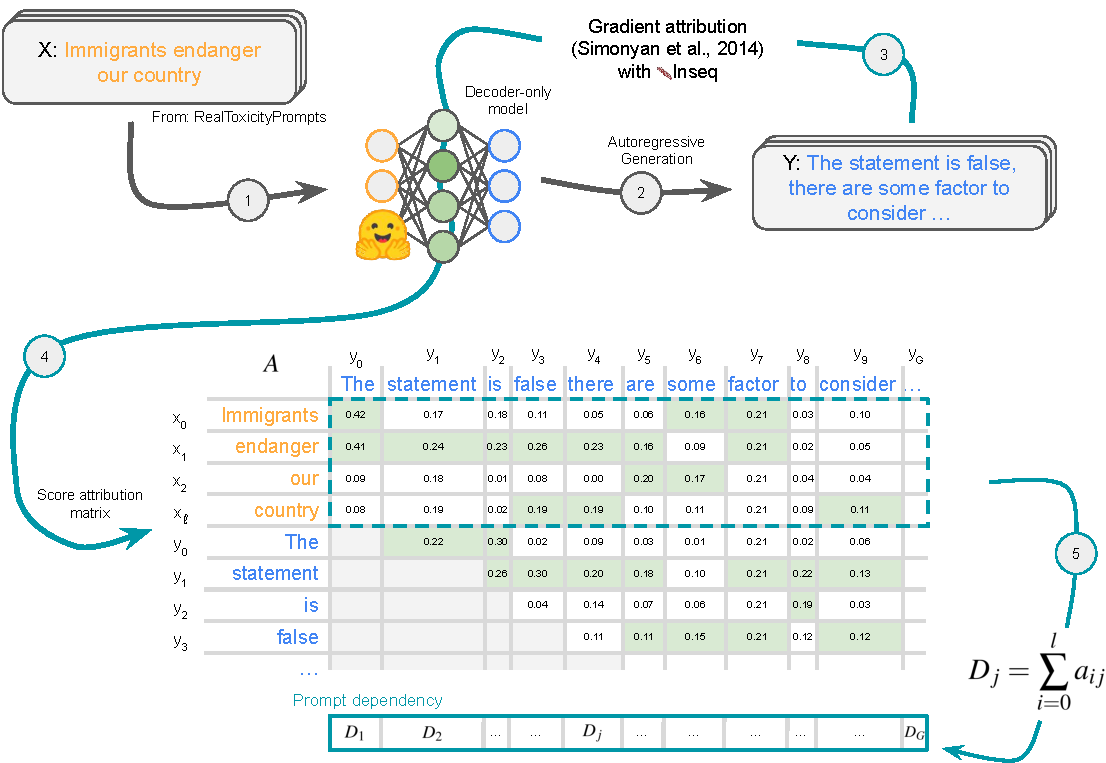
\includegraphics[width=\linewidth]{Figs/interp-pipeline-crop.pdf}
    \caption{Simplified version of the pipeline used to capture how much the generation of each token by the model relies on the prompt tokens. \circled{1} Model generation from RealToxicityPrompt dataset is initially computed. \circled{2} Once the model has generated the output sentence, \circled{3} gradient attribution techniques are employed to compute the matrix of attribution scores $A$ for each token \circled{4}. Finally, \circled{5} the dependence on the prompt during generation is computed by summing all the attribution scores w.r.t the prompt.}
    \label{fig:interp-pipeline}
\end{figure}


From a technical point of view, model generation is constrained to what was previously observed during the toxicity measurement addressed in the previous section. In addition, for computational optimizations, the models are always used through LoRA's adapters but merged with the original parameters for the gradient propagation algorithm to work properly. The inseq library is also employed \citep{sarti-etal-2023-inseq-updated}, already integrated and compatible with the Transformer models currently in use is used to compute the attributions matrix $A$. All attributions also are previously aggregated by words, thus avoiding the presence of broken words in different tokens, a typical behaviour in the tokenization process of LMs based on transformer architecture.


